\section{Results} \label{sc:results}

\ifIEEEtran
\else
We perform series of experiments to test the MDL description for the linear
manifold (LM) cluster described in section~\ref{sc:mdl-lmclus}.
Our first experiments are parametric experiments to illustrate the effect of
the number of precision bits carried and to understand the effect of
the error bound. The second experiment illustrates the results of the MDL linear
manifold clustering operating on different data sets.




First, we looked at how the quantization error $\varepsilon$ affects resulting
value of the MDL LM cluster description. We generated a 1D linear
manifold cluster, composed of 1000 points, in 2D Euclidean space where
points' coordinates where drawn from zero-mean normal distribution, independent
for every coordinate dimension.
In order to archive cluster shape compatible with 1D linear manifold, we used
different variances for each coordinate dimension. For $x$ coordinate,
the variance of the normal distribution is $\sigma_x = 1$ and for $y$ coordinate
$\sigma_y = 0.1$. Such cluster generation procedure creates a linear manifold
cluster, see Fig.~\ref{fig:lmc}, which is bounded in $x \in [-3;3]$ and
$y \in [-0.33;0.33]$.

\begin{figure}[ht]
\center
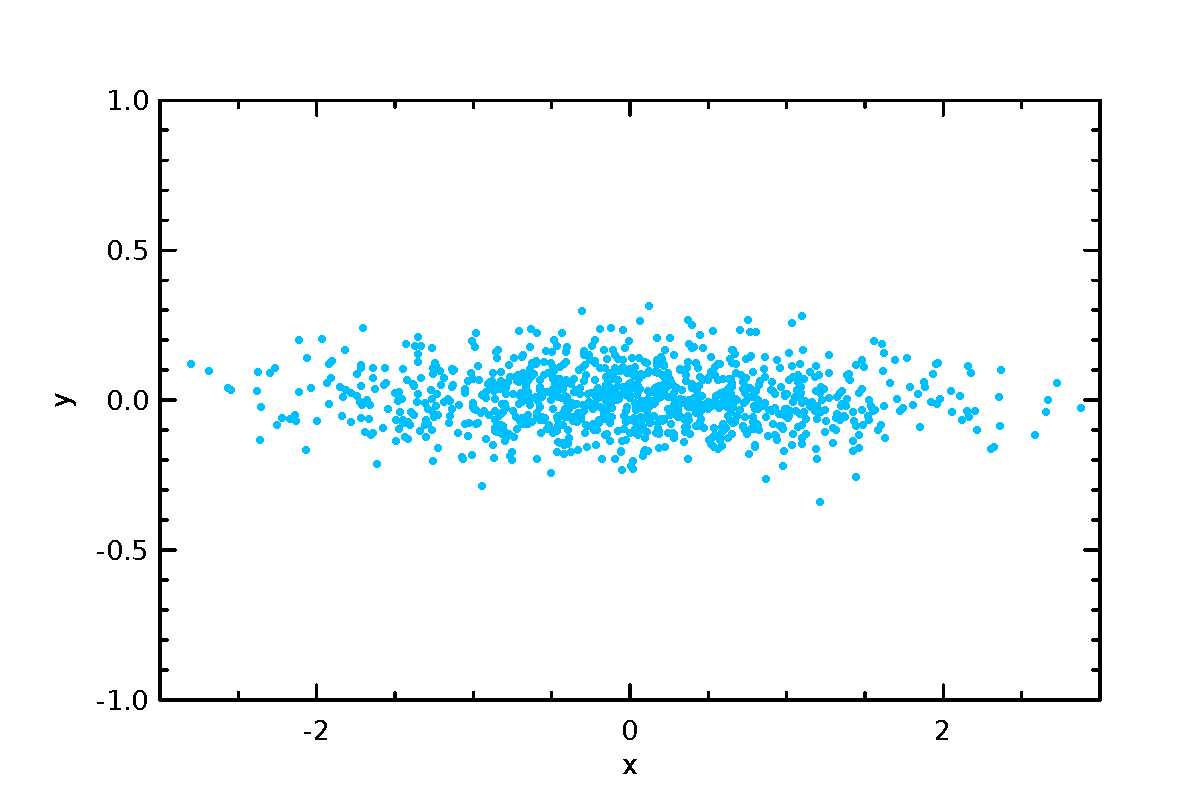
\includegraphics[width=3.5in]{img/results_lmc_1.pdf}
\caption{1D linear manifold cluster in 2D space}
\label{fig:lmc}
\end{figure}



For each quantization error $\varepsilon$, in range of values from $10^{-1}$ to
$10^{-8}$, we generate 100 LM clusters following above generation procedure and
calculate an average cluster MDL value and its 95\% confidence interval,
see Fig.~\ref{fig:mdl-exp1}. It is important to mention, there are two more
parameters involved in calculation of the cluster MDL value - model and data
encoding precision constants. These constants were set to 24 and 16 bits
accordingly.

% % Compose plots with subfigures (remove all figures fig:mdl-exp[1-2])
% \begin{figure}[ht]
% \hspace*{-60pt}
% \subfigure[]{
%     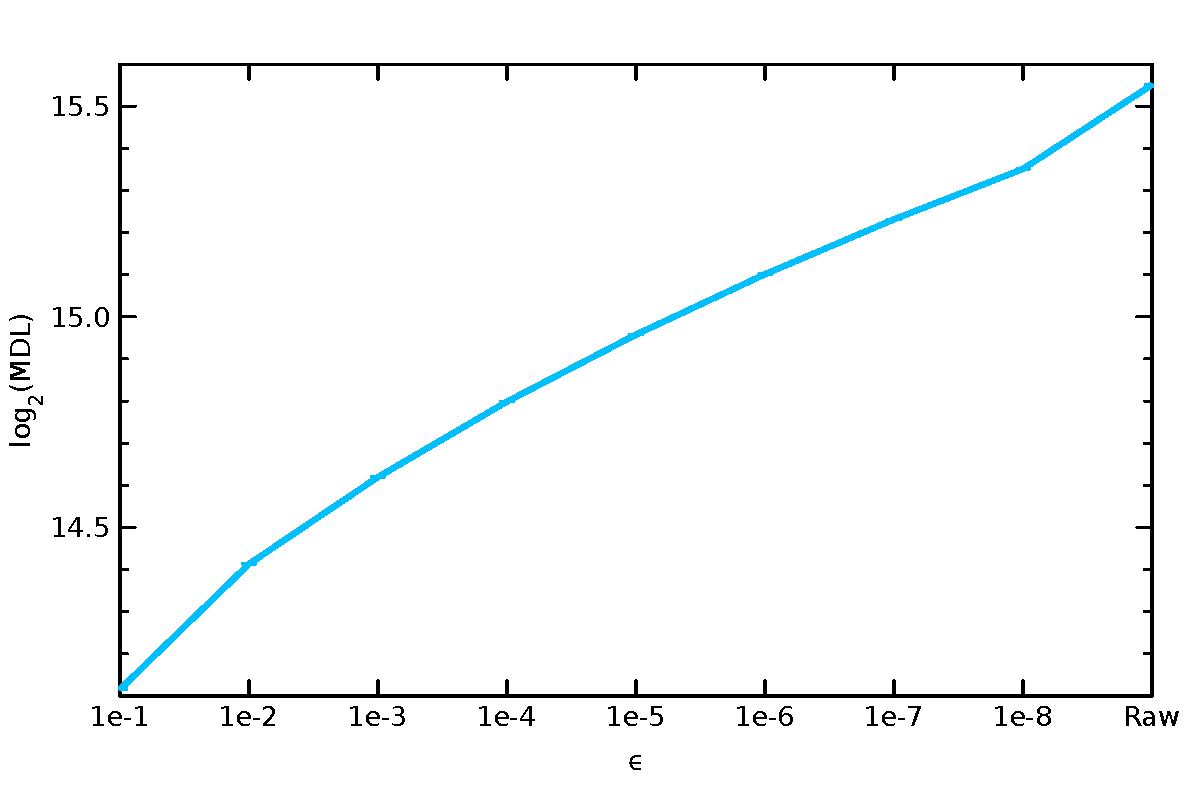
\includegraphics[width=3.5in]{img/results_mdl-exp1_1.pdf}
%    \label{fig:mdl-exp1}}
% \subfigure[]{
%     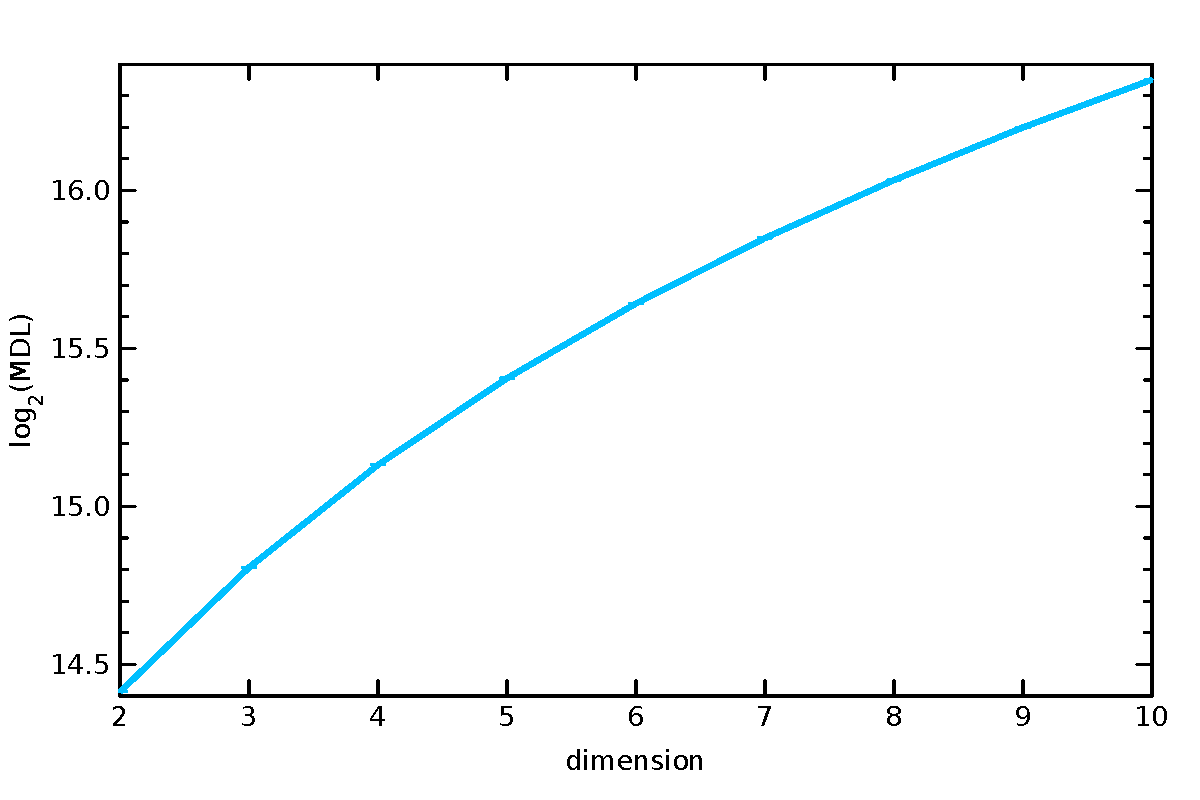
\includegraphics[width=3.5in]{img/results_mdl-exp2_1.pdf}
%     \label{fig:mdl-exp2}}
% \caption{
%     \subref{fig:mdl-exp1} MDL value of 1D LM cluster, in 2D space, calculated with quantization error \textepsilon; ``Raw'' value corresponds to the encoding without a model.
%     \subref{fig:mdl-exp2} MDL value of 1D LM cluster generated in a space of dimension from 2 to 10.
% }
% \end{figure}

\begin{figure}[ht]
\center
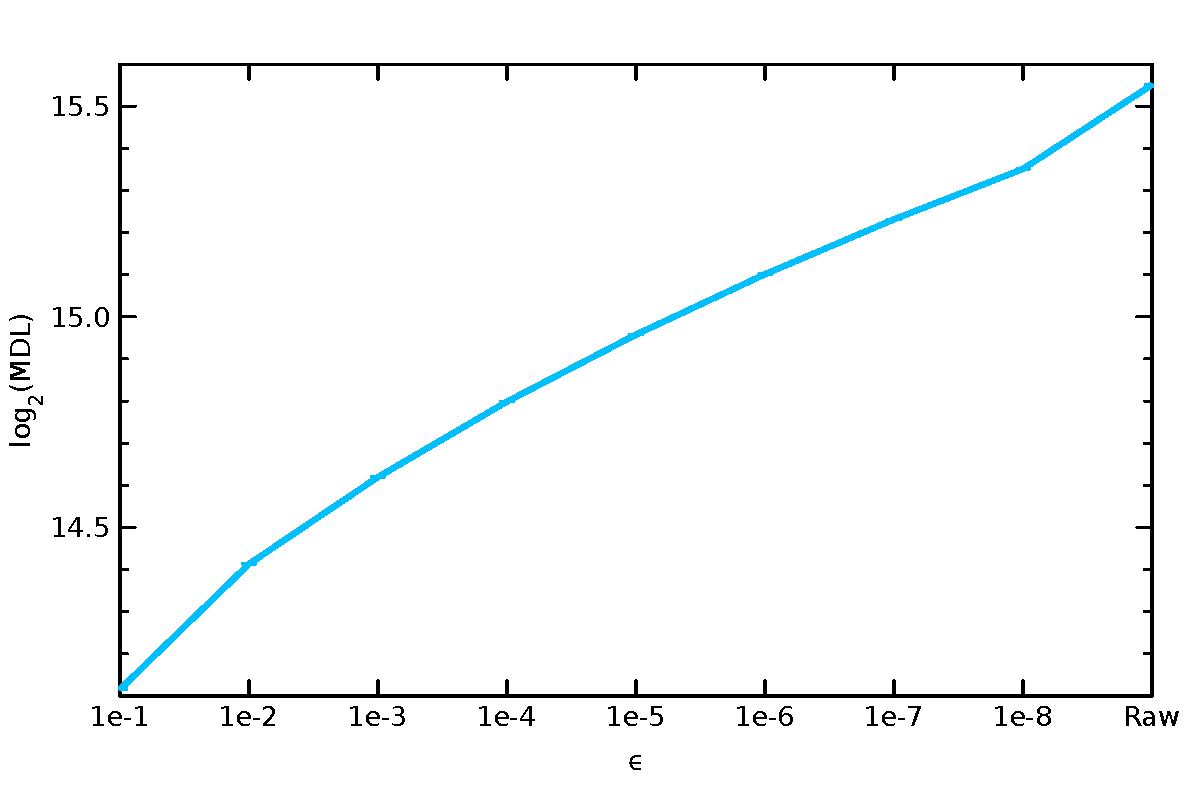
\includegraphics[width=4in]{img/results_mdl-exp1_1.pdf}
\caption{MDL value of 1D linear manifold cluster, in 2D space, calculated with quantization error \textepsilon. ``Raw'' value corresponds to the encoding without a model.}
\label{fig:mdl-exp1}
\end{figure}



As expected, while the quantization error decreased, there was a more
precise encoding of point distribution in the orthogonal complement space of the
cluster manifold and  the corresponding MDL value of the LM cluster increased
up to the maximum possible value of uncompressed raw encoding.
\bigskip
%
Next, we investigated dependency of the MDL value on the LM cluster dimension. We
calculated MDL values of a 1D linear manifold cluster in full space of dimension
from 2 to 10. In order to generate 1D LM cluster for high dimensional spaces,
we used same methodology as with a 2D space, first coordinate was generated from
normal distribution with variance 1.0, the rest of the coordinates were drawn
from normal distribution with variance 0.1. We used same encoding constants as
in previous experiment, and the value of quantization error was set to 0.01.

As we expected, the MDL value of the 1D LM cluster would increase with number of
space dimensions. This is shown in Fig.~\ref{fig:mdl-exp2}.
\bigskip

\begin{figure}[ht]
\center
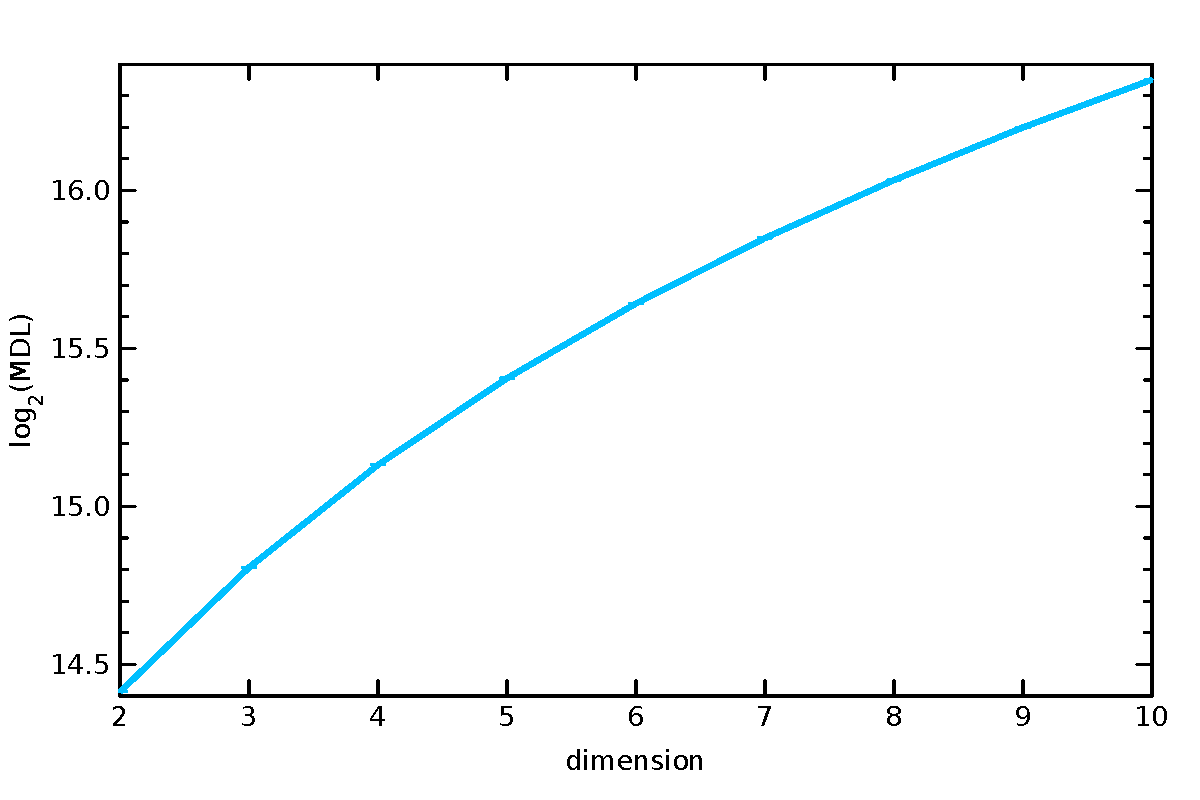
\includegraphics[width=4in]{img/results_mdl-exp2_1.pdf}
\caption{MDL value of 1D linear manifold cluster generated in a space of dimension from 2 to 10.}
\label{fig:mdl-exp2}
\end{figure}



Also, we investigated the dependency of the MDL value of LM cluster as
the encoding precision constants changes. In above experiments, we use values of
24 and 16 for the model and data encoding precision constants. We varied these
pair of constant for calculation of MDL value for a 1D LM cluster in 2D space.


% % Compose plots with subfigures (remove all figures fig:mdl-exp[3-4])
% \begin{figure}[ht]
% \hspace*{-50pt}
% \subfigure[]{
%     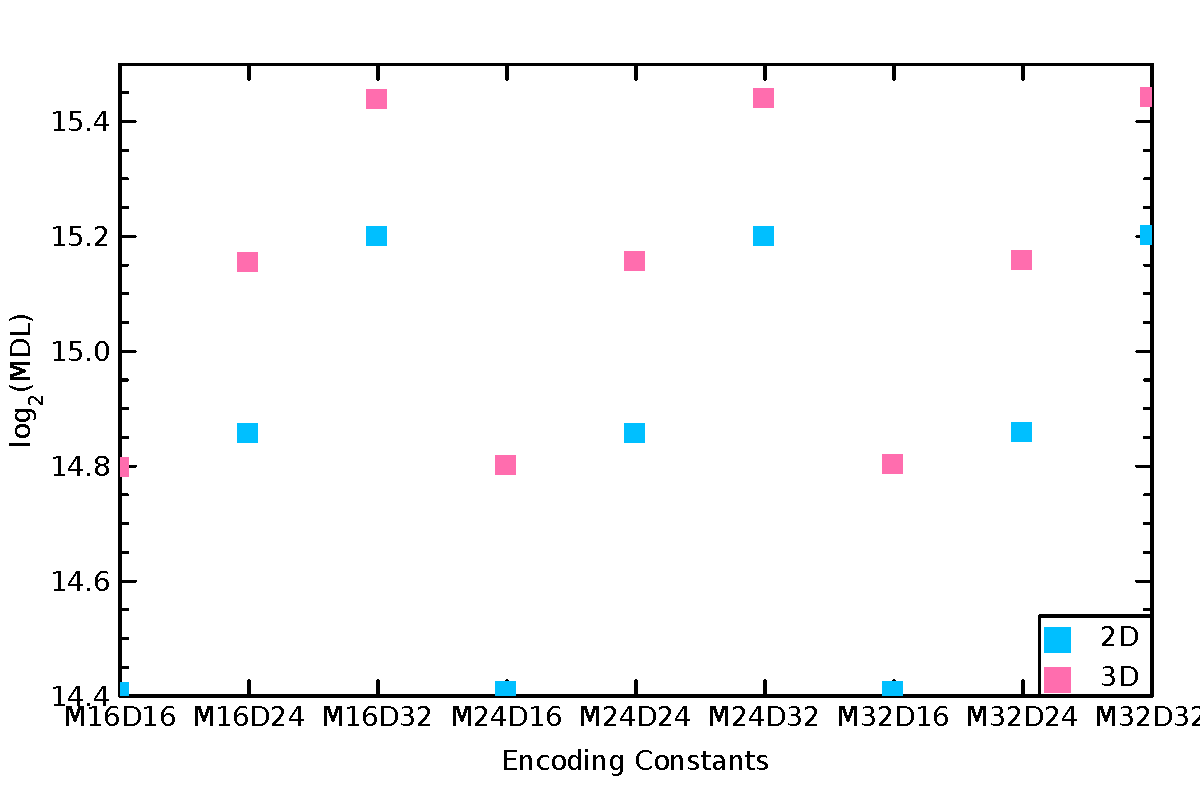
\includegraphics[width=3.5in]{img/results_mdl-exp3_1.pdf}
%     \label{fig:mdl-exp3}}
% \subfigure[]{
%     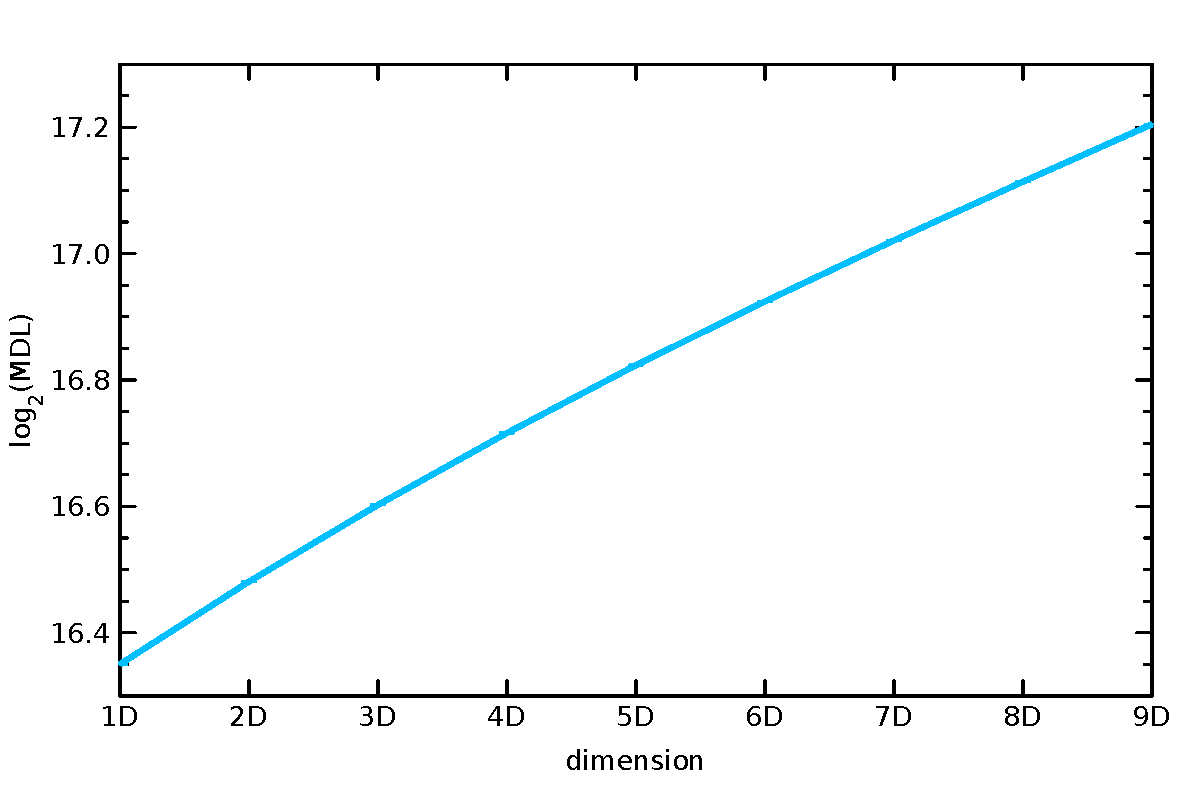
\includegraphics[width=3.5in]{img/results_mdl-exp4_1.pdf}
%     \label{fig:mdl-exp4}}
% \caption{
%     \subref{fig:mdl-exp3} MDL value of 1D LM cluster in 2D space w.r.t. encoding constants (\emph{EConst} axis shows values of encoding constants as \emph{m[I]d[J]} where $I$ is model constant value and $J$ is data constant value).
%     \subref{fig:mdl-exp4} MDL values of LM clusters with dimensions from 1 to 9 in 10D space.
% }
% \end{figure}

\begin{figure}[H]
\center
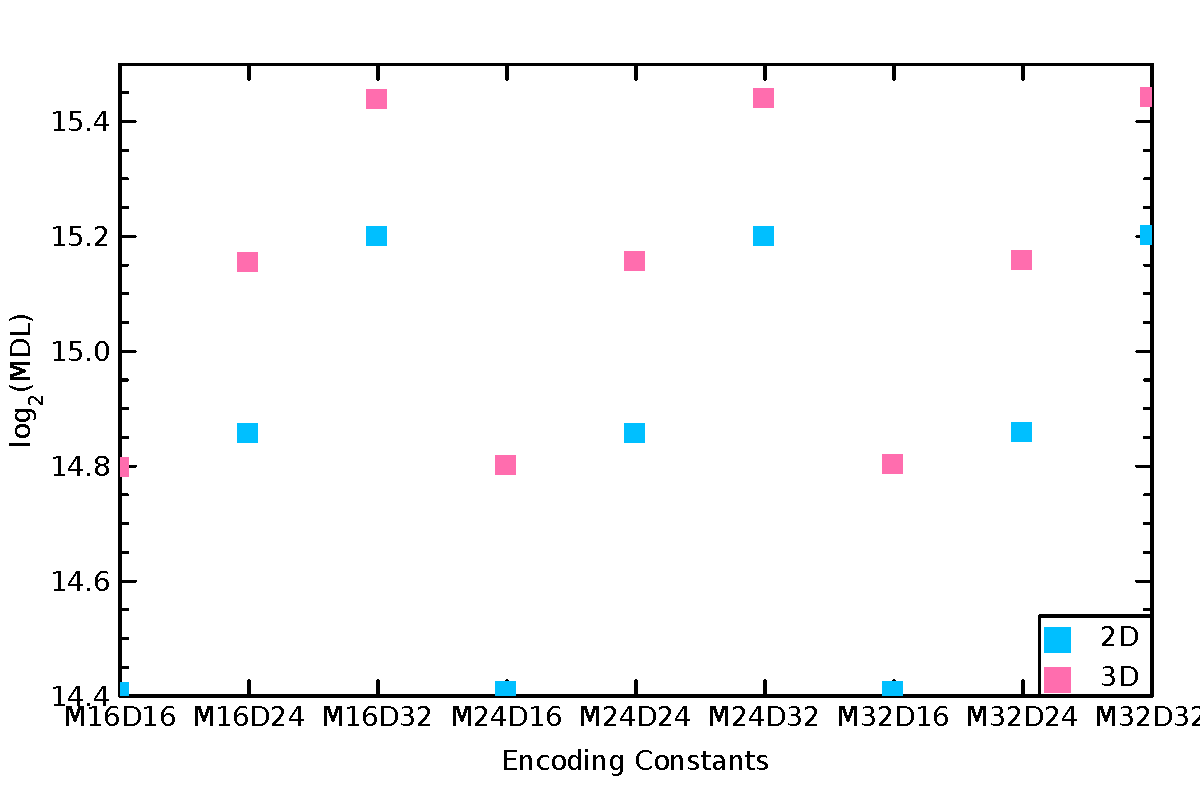
\includegraphics[width=4in]{img/results_mdl-exp3_1.pdf}
\caption{MDL value of 1D linear manifold cluster in 2D space w.r.t. encoding constants (\emph{Encoding Constants} axis shows values of encoding constants as \emph{M[I]D[J]} where $I$ is model constant value and $J$ is data constant value).}
\label{fig:mdl-exp3}
\end{figure}



Fig.~\ref{fig:mdl-exp3} shows that the model encoding constant does not
contribute much to overall value of the cluster MDL. For 1D linear manifolds in
2D and 3D space, the main factor which affects the resulting MDL value is
the data encoding precision constants.
\bigskip
\fi

% LM type: Compare 1D and 2D LM cluster in 3D
\ifIEEEtran
\else
The following experiment allows us to determine how the dimensionality of
the LM cluster affects the calculation of its MDL value. We create multiple
linear manifolds with increasing dimension in a 10 dimensional space. LM cluster
generation is done in a standard way: generate coordinate values of the cluster
points from a normal distribution. For a primary dimension of the LM cluster,
the variance is 1.0, and for dimensions in the orthogonal complement to
the linear manifold, the variance is set to 0.1. The encoding constants,
model and data, are 24 and 16. The quantization error bound is set to 0.01.

\begin{figure}[H]
\center
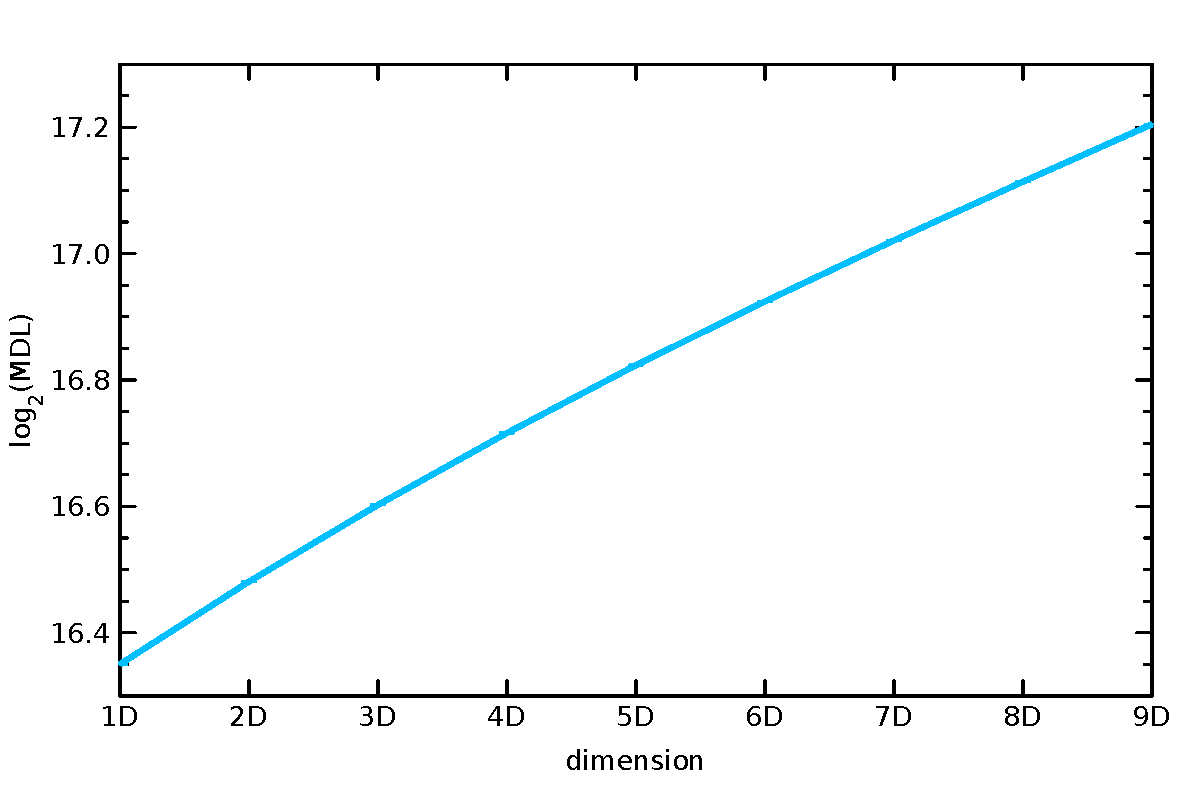
\includegraphics[width=4in]{img/results_mdl-exp4_1.pdf}
\caption{MDL values of LM clusters with dimensions from 1 to 9 in 10D space.}
\label{fig:mdl-exp4}
\end{figure}



Fig.~\ref{fig:mdl-exp4} shows expected linear growth of the MDL value with
the manifold dimensionality which is reflected in first term
of (\ref{eq:mdl-lmc-data}). More coordinates are encoded with constant factor
$P_d$ which is overpowering entropy term of coordinates in the orthogonal
complement space of the LM cluster.
\fi

% Take a J-dimensional manifold cluster and calculate MDL as if cluster dim != J
Finally, we would like to understand how well MDL evaluates goodness of
a linear manifold cluster. Suppose, we have a 2D linear manifold cluster in
3D space. How can we guarantee that the particular cluster is actually
a 2D cluster? What if this cluster is 1D linear manifold cluster with
wide bounds? What will be the criteria which would provide a distinctive answer
on correctness of a structure description of the linear manifold cluster.
We claim that MDL value of linear manifold cluster, calculated with correct
assumptions of the linear manifold cluster structure would yield minimal value.

In order to test above assumption, we generated a 5D linear manifold cluster in
a 10D space, following a similar cluster generation schema as in above experiments.
We generated coordinate values of the cluster points from a normal distribution,
where for a primary dimension of the LM cluster, the variance is set 1.0, and
for dimensions in the orthogonal complement to the linear manifold, the variance
is set to 0.1. The encoding constants, model and data, are 24 and 16.

We calculated the MDL value of this cluster as if its dimension is unknown
to us, as it happens during a selection of the cluster candidate manifold
in LMCLUS algorithm. We specify during the MDL value calculation that our
5D cluster has dimension in range from 1 to 9. Moreover, we use various
quantization errors during this experiment to understand how precision of
the cluster description affects goodness of the selected cluster structure.

\begin{figure}[ht]
\center
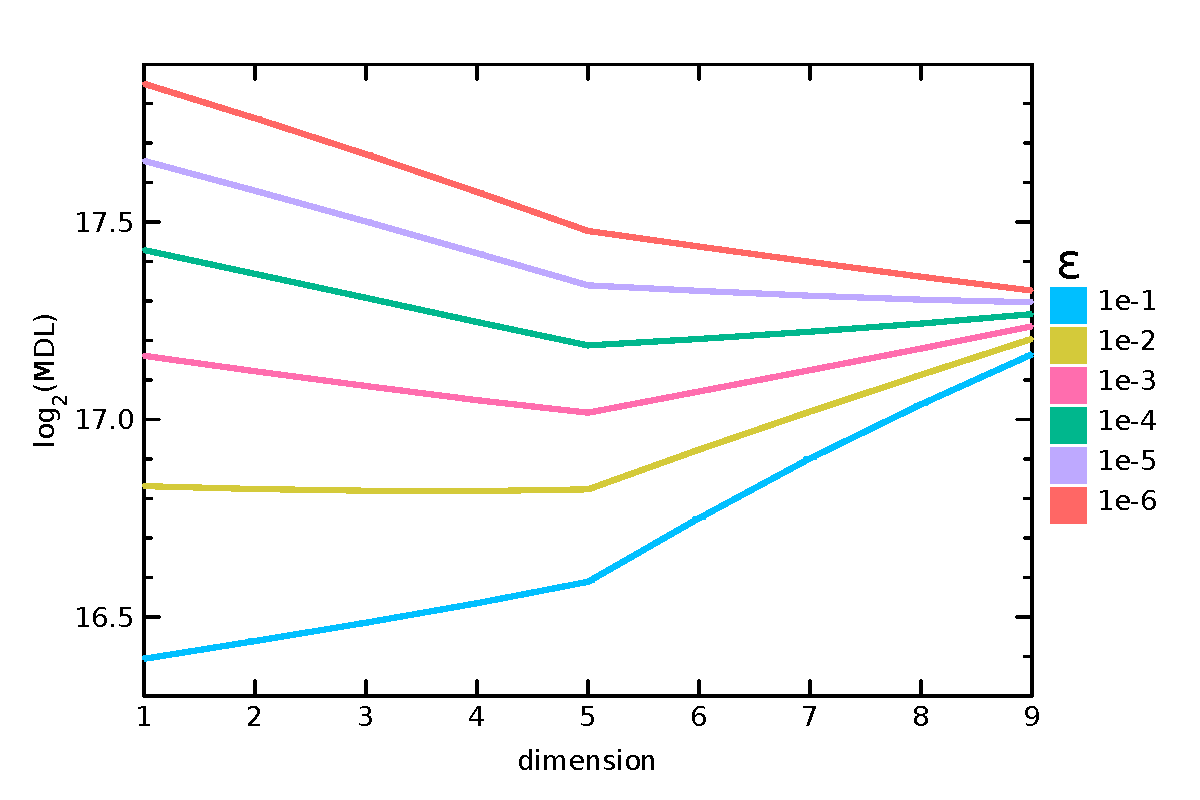
\includegraphics[width=\IfClass{IEEEtran}{3.5in}{4in}]{img/results_mdl-exp5_1.pdf}
\caption{MDL values, calculated with various cluster dimensionality parameters and quantization error \textepsilon for a cluster that is actually a 5D LM cluster in a 10D space.}
\label{fig:mdl-exp5}
\end{figure}



Fig.~\ref{fig:mdl-exp5} shows that MDL value calculated with correct structural
parameters of the examined linear manifold cluster has minimum value when
the dimension parameter corresponds to the cluster dimensionality.
As we established before, see Fig.~\ref{fig:mdl-exp1}, low values of
the quantization error $\varepsilon$ will result in the high cluster MDL value.
High values of $\varepsilon$  will result in the low cluster MDL value.
If the quantization error $\varepsilon$ set to small value, the cluster MDL
value will decreases monotonically with the dimension of cluster.
If the quantization error $\varepsilon$ set to large value, the cluster MDL
value will increases monotonically with the dimension of cluster.
If the quantization error $\varepsilon$ set correctly, the cluster MDL
value will decreases until the right number of dimensions is selected after
which MDL value increases with increasing number of dimension parameter.

% However, when the cluster dimension considered to be lower then the actual one,
% some of the constrained dimensions forced to be quantized. This leads to
% the smaller entropy value in comparison to the proper encoding of the cluster
% when the quantization error is high, or to large values when the quantization
% error is low.
% Similar situation arise when the cluster dimension considered to be higher then
% the actual one, so some unconstrained dimensions are forced to constant encoding
% rather then quantization which results in the larger MDL value in comparison to
% the proper encoding.
